\phantomsection
\section*{4. More Topological Spaces}
\addcontentsline{toc}{section}{4. More Topological Spaces}

\phantomsection
\subsection*{1. Metric Topological Spaces}
\addcontentsline{toc}{subsection}{1. Metric Topological Spaces}

\begin{customdefinition}{4.1}[Metric]
A metric on a set $X$ is a function 
$d: X \times X \longrightarrow \R$
such that 
\begin{enumerate}
    \item[1).] $d(x,y)\geqslant 0$ with equality if and only if $x =y$
    \item[2).] $d(x,y) = d(y,x)$
    \item[3).] (Triangle equality) $d(x,y) + d(y,z) \geqslant d(x,z)$
\end{enumerate}
for all $x, y, z, \in X$.
\end{customdefinition}

\begin{customthm}{4.1}
Let $X$ be a set with metric $d$. Then the collection
$$\B_d = \left\{B_{\epsilon}(x;d) \mid x\in X, \epsilon > 0\right\}$$
is a basis for a topology on $X$, called the metric topology induced by $d$.
\end{customthm}

\begin{proof}
Since $d(x,x) = 0$, we see that $x\in B_{\epsilon} (x;d)$ for every $\epsilon > 0$. So, $\B_{d}$ covers $X$.\\
Let $B_{\epsilon_1}(x_1), B_{\epsilon_3}(x_2) \in \B_{d}$ with 

    $$y \in B_{\epsilon_1}(x_1) \cap B_{\epsilon_3}(x_2)$$
    
    Let $\delta_1 = \epsilon_1 - d(x_1,y)$. If $z \in B_{\delta_1}(y)$, then 
    
    \begin{minipage}{0.5\textwidth}
    \begin{align*}
        d(x,z) & \leqslant d(x,y) + d(y,z)\\
                &< d(x,y) + \epsilon_1 - d(x,y)\\
                &< \epsilon_1\\
    \end{align*}
    \end{minipage}\begin{minipage}{0.5\textwidth}
    \begin{center}
    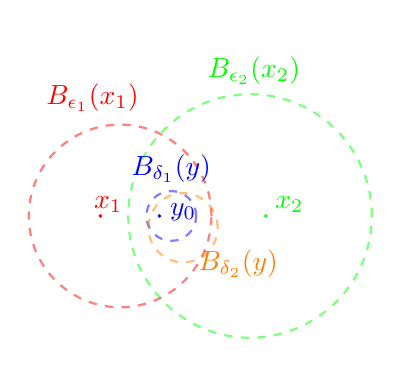
\begin{tikzpicture}[scale = 0.5]
    \draw[red, semitransparent, dashed, thick] (-1,0) circle[radius=66pt];
    \node[label, red] at (-1.7,3) {$B_{\epsilon_1}(x_1)$};
    \node[label, red] at (-1.3, 0.3) {$x_1$};
    \node[circle, fill, red, inner sep=0.5pt] at (-1.5, 0) {};
    \draw[green, semitransparent, dashed, thick] (2.3,0) circle[radius=88pt];
    \node[label, green] at (2.4, 3.7) {$B_{\epsilon_2}(x_2)$};
    \node[label, green] at (3.3, 0.3) {$x_2$};
    \node[circle, fill, green, inner sep=0.5pt] at (2.7, 0) {};
    \draw[blue, semitransparent, dashed, thick] (0.3,0) circle[radius=18pt];
    \node[label, blue] at (0.3, 1.2) {$B_{\delta_1}(y)$};
    \node[label, blue] at (0.6, 0.1) {$y_0$};
    \node[circle, fill, blue, inner sep=0.5pt] at (0, 0) {};
    \draw[orange, semitransparent, dashed, thick] (0.6,-0.3) circle[radius=25pt];
    \node[label, orange] at (2, -1.2) {$B_{\delta_2}(y)$};
    \end{tikzpicture}
    \end{center}
    \end{minipage}
    
    so that $B_{\delta_1}(y) \subset B_{\epsilon_1}(x_1)$. Similarly, setting $\delta_2 = \epsilon_2 - d(x_2, y)$ gives $B_{\delta_2}(y) \subset B_{\epsilon_2}(x_2)$. Let
        $$\delta = \text{min}\left\{\delta_1, \delta_2\right\}$$
    Then
    $$B_{delta}(y) \subset B_{\epsilon_1}(x_1) \cap B_{\epsilon_2}(x_2)$$
\end{proof}

\begin{customdefinition}{4.2}[Metrizable]
A topological space $X$ is called metrizable if there exists a metric $d$ on $X$ whose associated metric topology agrees with that of $X$.\\
Metrizability of a topological space is a subtle problem, but is ultimately known via Urysohn's Metrization Theorem.
\end{customdefinition}

\begin{customdefinition}{4.3}
Let $(X, d)$ be a metric space.
\begin{enumerate}
    \item[1).] A subset $A \subset X$ is called bounded if there exists an $N>0$ such that $d(a_1, a_2) \leqslant N$ for all $a_i \in A$.
    \item[2).] The diameter of a non-empty bounded subset $A\subset X$ is 
                $$\text{diam} A = \text{sup} \left\{d(a_1, a_2) \mid a_i \in A\right\}.$$
\end{enumerate}
\end{customdefinition}

\begin{customthm}{4.2}
Let $(X, d)$ be a metric space. Then define $\overline{d}: X\times X \longrightarrow \R$ by
    $$\overline{d} = \text{min} \left\{d(x,y), 1\right\}$$
in other words
    \begin{align*}
        \overline{d}: X\times X &\longrightarrow \R\\
        (x,y) &\longrightarrow \text{min} \left\{d(x,y), 1\right\}
    \end{align*}
Then $\overline{d}$ is a metric that includes the same topology as $d$.
\end{customthm}

\begin{customthm}{4.3}
The following statements hold.
\begin{enumerate}
    \item[1).] Subspaces of metric space are metrizable.
    \item[2).] Metrizable spaces are Hausdorff.
\end{enumerate}
In particular, Lemma $2.19$ and the $2)$ imply that, if a sequence $x_n$ in a metric space converges, then if has a unique limit.
\end{customthm}

\begin{proof}
\begin{enumerate}
    \item[1).] Let $(X, d)$ be a metric space and $A \subset X$ a subspace. We claim that
                $$d_{\vert A}: A \times A \longrightarrow \R$$
                is a metric on $A$ and that the metric topology on $A$ agrees with the subspace topology. That $d_{\vert A}$ is a metric follows immediately from the metric axioms hold. For the second, we wish to apply Lemma $2.3$. Let
                $$\mathcal{A} =\left\{\underbrace{B_{\epsilon}(y)}_{\text{ with respect to $d_{\vert A}$}} \subset Y \mid y \in Y,\, \epsilon > 0\right\}$$
                (This is the set $\mathcal{C}$ in Lemma $2.3$). Note that 
                $$B_{\epsilon}(y) = \underbrace{B_{\epsilon}}_{\text{open in $X$}}\left(y;d\right) \cap Y$$
                So that $B_{\epsilon}(y) \subset Y$ is open. Let $U \subset Y$ be open and $u \in U$. Then
                $$U = \underaccent{i}{\bigcup}\left(B_{\epsilon_i}(x_i, d) \cap Y\right)$$
                for some $i$. Then 
                $$u \in B = B_{\epsilon_i - d(x_i, u)}(u) \subset U.$$
                Lemma $2.3$ therefore applies, proving the second statement.
    \item[2).] Let $(X, d)$ be a metric space and $x, y \in X$ distinct points. Let $\epsilon = d(x,y) >0$(by the non-negativity axiom). Then $x \in B_{\epsilon/2}(x)$ and $y \in B_{\epsilon/2}(y)$ and 
                $$B_{\epsilon/2}(x) \cap B_{\epsilon/2}(y) = \varnothing$$
                (by the Triangle Inequality). So, $(X,d)$ is Hausdorff.
\end{enumerate}
\end{proof}

\begin{customthm}{4.4}
Finite products of metrizable topological spaces are metrizable.
\end{customthm}

\begin{customthm}{4.5}
Let $(X, d)$ and $(Y, e)$ be metric spaces. A function $f: X \longrightarrow Y$ is continuous if and only if for each $x \in X$ and $\epsilon >0$, there exists a $\delta >0$ such that 
        $$e\left(f(x), f(y)\right) < \epsilon$$
    whenever $d(x,y) < \delta$.\\
    In other words,
        $$d_{X}(x,y) < \delta \implies d_{Y} \left(f(x), f(y)\right) < \epsilon$$
Continuous functions between metric spaces admit an $\epsilon - \delta$ characterization, just like in analysis.
\end{customthm}

\begin{customlemma}{4.6}
Let $A \subset X$ be a subset of a topological space.
\begin{enumerate}
    \item[1).] If $\left\{x_n\right\}_{n \geqslant 0}$ is a sequence in $A$ converging to a point $x$, then $x \in \overline{A}$.
    \item[2).] If $X$ is metrizable and $x \in \overline{A}$, then there exists a sequence $\left\{x_n\right\}_{n \geqslant 0}$ in $A$ converging to $x$.
\end{enumerate}
\end{customlemma}

\begin{customthm}{4.7}
Let $f: X \longrightarrow Y$ be a function between topological spaces.
\begin{enumerate}
    \item[1).] If $f$ is continuous and $\left\{x_n\right\}_{n \geqslant 1}$ converges to $x$, then $\left\{f(x_n)\right\}_{n \geqslant 1}$ converges to $f(x)$.
    \item[2).] If $X$ is metrizable $\left\{f(x_n)\right\}_{n \geqslant 1}$ converges to $f(x)$ for all sequences ${x_n}_n$ converging to $x$, then $f$ is continuous.
\end{enumerate}
\end{customthm}

\newpage

\begin{proof}
\begin{enumerate}
    \item[1).] Let $\left\{x_n\right\}_{n \geqslant 1}$ converges to $x \in X$ and $U \subset Y$ be an open set containing $f(x)$. Since $f$ is continuous, $f^{-1}(U) \subset X$ is open and, by construction, contains $x$. Hence, there exists an $N>0$ such that $x_n \in f^{-1} (U)$ whenever $n >N$. But then $f(x_n) \in U$ whenever $n>N$. So, $\left\{f(x_n)\right\}_{n \geqslant 1}$ converges to $f(x)$.
    \item[2).] Let $(X, d)$ be a metric space and $\left\{x_n\right\}_{n \geqslant 1}$ a convergent sequence, say $x = \displaystyle\lim_{n \to \infty} x_n$. (Note: Since $X$ is metrizable, $\left\{x_n\right\}_{n \geqslant 1}$ converges to a unique point, so that we can safely write $\displaystyle\lim_{n \to \infty} x_n$).\\
    Recall that $f$ is continuous if and only if 
    $$f\left(\overline{A}\right) \subset \overline{f(A)}$$
    for all $A\subset X$; see Theorem $3.2$. Let $x\in \overline{A}$. By Lemma $4.6$, there exists $\left\{x_n\right\}_{n \geqslant 1}$ with $x = \displaystyle\lim_{n \to \infty} x_n$. By hypothesis, $\left\{f(x_n)\right\}_{n \geqslant 1}$ converges to $f(x)$, that is, $f(x) \in \overline{f(A)}$, again by Lemma $4.6$.
\end{enumerate}
\end{proof}

\begin{customdefinition}{4.4}
Let $(X, d)$ be a metric space.
\begin{enumerate}
    \item[1).] A sequence $\left\{x_n\right\}_{n \geqslant 1}$ is called Cauchy if for all $\epsilon > 0$ there exists an $N > 0$ such that 
                $$d(d_n, d_{n+1}) < \epsilon$$
                whenever $m, n > N$
    \item[2).] $(X, d)$ is called complete if every Cauchy sequence converges.
\end{enumerate}
\end{customdefinition}

\begin{customexa}{4.1}The following are examples about complete metric space.
\begin{enumerate}
    \item[1).]$\left(\R, d_E\right)$ is complete;
    \item[2).]$(0,1)$ is not complete, for example
    $$\left\{\dfrac{1}{n}\right\}_{n \geqslant 1}\text{ is Cauchy but does not converge in }(0,1).$$
\end{enumerate}
\end{customexa}

\phantomsection
\subsection*{2. The Quotient Topology}
\addcontentsline{toc}{subsection}{2. The Quotient Topology}

\begin{customdefinition}{4.5}[Equivalence Relationship]
Let $X$ be a set. An equivalence relation on $X$ is $x \sim y$, such that
\begin{enumerate}
    \item[1).] (Reflexivity) $x \sim x$, 
    \item[2).] (Symmetry) $x \sim y$ if and only if $y \sim x$,
    \item[3).] (Transitivity) If $x \sim y$ and $y \sim z$, then $x \sim z$.
\end{enumerate}
The equivalence class of $x$ is 
$$[x] = \left\{y \in X \mid x \sim y\right\} \subset X$$
So 
$$X = \underaccent{x \in X/\sim}{\bigsqcup}[x]$$ 
where $X/\sim = \left\{\text{set of all equivalence classes}\right\}$.
\end{customdefinition}

\begin{customdefinition}{4.6}[Quotient Topology]
Let $X$ be a topological space, $Y$ a set and 
$$q: X\longrightarrow Y$$
a surjective function. The quotient topology on $Y$ (induced by the function $q$) is 
$$\tau_q = \left\{U \subset Y \mid q^{-1}(U) \subset X \text{ is open }\right\}$$
We call $(Y, \tau_q)$ the quotient topological space.\\
\end{customdefinition}

\begin{proof}
We should check this is indeed a topology:
\begin{enumerate}
    \item[1.)] $\varnothing \in \tau_q$ because $q^{-1}(\varnothing) = \varnothing \in \tau$ (topology on $X$). And $Y \in \tau_q$ because $q^{-1}(Y) = X \in \tau$ ($q$ is surjective.)
    \item[2.)] Let $\{U_i\}_{i\in I}$ be an arbitrary collection in $\tau_q$. Then 
    $$q^{-1}\left(\underaccent{i \in I}{\bigcup}U_i\right) = \underbrace{\underaccent{i \in I}{\bigcup} \underbrace{q^{-1}\left(U_i\right)}_{\text{ open in }X}}_{\text{ open in} X} \in \tau_q$$
    \item[2.)] Let $\{U_i\}_{i\in I}$ be a finite collection in $\tau_q$. Then 
    $$q^{-1}\left(\underaccent{i \in I}{\bigcap}U_i\right) = \underbrace{\underaccent{i \in I}{\bigcap} \underbrace{q^{-1}\left(U_i\right)}_{\text{ open in }X}}_{\text{ open in} X} \in \tau_q$$
\end{enumerate}
\end{proof}

\begin{customexa}{4.2}Let $X = \R$. Define an equivalence relation on $X$ by
    $$x \sim y \iff x - y \in \mathbb{Q}$$
    Consider the quotient $X/\sim$. The points $[0], [\pi] \in X/\sim$ are distinct. Let
    $$[0] \in U, \,\, [\pi] \in V$$
    be open sets in (in $X/\sim$). Then $q^{-1}(U) \subset \R$ is an open set which contains $\mathbb{Q}$ and $q^{-1}(V) \subset \R$ is an open set which contains 
    $$\pi + \mathbb{Q} = \left\{\pi + r \mid r \in \mathbb{Q}\right\}$$
    But then $q^{-1}(U) \cap q^{-1}(V) \neq \varnothing$. So, $U \cap V \neq \varnothing$, and $X/\sim$ is not Hausdorff. This example shows that quotient spaces do not, in general inherit the Hausdorff property.
\end{customexa}

\begin{customdefinition}{4.7}[Quotient Map]
Let $X$ and $Y$ be topological spaces; let $f: X\longrightarrow Y$ be a surjective map. The map $f$ is said to be a quotient map provided a subset $U$ of $Y$ is open in $Y$ if and only if $p^{-1}(U)$ is open in $X$.
\end{customdefinition}

\begin{customdefinition}{4.8}[Saturated]
Let $f: X \longrightarrow Y$ be a surjective map of topological spaces. A subset $S \subset X$ is called saturated (with respect to $f$) is any $y \in Y$ which satisfies 
$$S \cap f^{-1}\left(\{y\}\right) \neq \varnothing$$
also satisfies 
$$f^{-1}\left(\{y\}\right) \subset S$$
\emph{Book:} We say that a subset $C$ of $X$ is saturated (with respect to the surjective map $p: X\longrightarrow Y$) if $C$ contains every set $p^{-1} \left(\{y\}\right)$ that it intersects. Thus $C$ is saturated if it equals the complete inverse image of a subset of $Y$. To say that $p$ is a quotient map is equivalent to saying that $p$ is continuous and $p$ maps \emph{saturated} open sets of $X$ to open sets of $Y$ (or saturated closed sets of $X$ to closed sets of $Y$).\\
\emph{More:} A set $X$ is saturated if
    $$S = \underaccent{y\in q(S)}{\bigcup}f^{-1}\left(\{y\}\right)$$
\end{customdefinition}

\begin{customlemma}{4.8}
Let $q: X \longrightarrow Y$ be a continuous surjection. Then $q$ is a quotient map if and only if whenever $V \subset X$ is open and saturated, $q(V) \subset Y$ is open.
\end{customlemma}

\begin{proof}It's another if-and-only-if, you know the drill...
\begin{enumerate}
    \item[$\Longrightarrow$: ] Assume that $q$ is a quotient map. Then $q$ is continuous. Let $V \subset X$ be open and saturated. We claim that
    $$V = q^{-1}\left(q(v)\right)$$
    Clearly, $V \subset q^{-1}\left(q(v)\right)$. Let $x \in q^{-1}\left(q(v)\right)$, that is, $q(x) \in q(v)$. Then $q^{-1}\left(q(x)\right) \cap V \neq \varnothing$. Since $V$ is saturated, $q^{-1}\left(q(v)\right) \subset V$. Or
    $$V = \underaccent{y\in q(V)}{\bigcup}q^{-1}\left(\{y\}\right)$$
    So that 
    $$V = q^{-1}\left(q(v)\right)$$
    Since $q$ is a quotient map and $q^{-1}\left(q(v)\right)$ is open, we know $q\left(V\right) \subset Y$ is open.
    
    \item[$\Longleftarrow$: ]Assume that $q$ is continuous and, if $V \subset X$ is open and saturated, then $q(V)$ is open . Let $U \subset Y$ be a subset such that $q^{-1}(U)$ is open; we need to show that $U \subset Y$ is open. Since $q\left(q^{-1}(U)\right) = U$, it suffices to show that $q^{-1}(U)$ is saturated. Say $y \in Y$ satisfies $q^{-1}\left(\{y\}\right) \cap q^{-1}(U) \neq \varnothing$. Then $y \in U$ and $q^{-1}\left(\{y\}\right) \subset q^{-1}(U)$
\end{enumerate}
\end{proof}

\begin{customthm}{4.9}
Let $g: X \longrightarrow Y$ be a quotient map and $Z$ a topological space. If $f: X \longrightarrow Z$ is continuous and takes a single value in each $g^{-1}\left(\{y\}\right)$, $y \in Y$, then $f$ determines a (unique) continuous function
$$\widetilde{f}: Y \longrightarrow Z$$
such that 
$$f: \widetilde{f} \circ g$$
In pictures:
    \begin{center}
    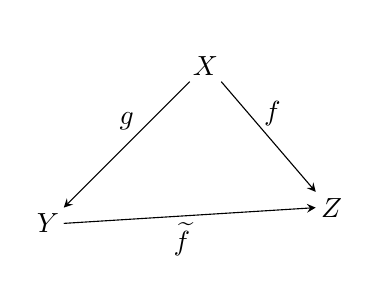
\begin{tikzpicture}
    \node[label] at (0,1) {$X$};
    \node[label] at (1.6,-0.8) {$Z$};
    \node[label] at (-2,-1) {$Y$};
    \draw[-stealth](0.2,0.8) -- (1.4,-0.6);
    \draw[-stealth](-0.2,0.8) -- (-1.8,-0.8);
    \draw[-stealth](-1.8,-1) -- (1.4,-0.8);
    \node[label] at (0.85,0.4) {$f$};
    \node[label] at (-1,0.3) {$g$};
    \node[label] at (-0.3,-1.2) {$\widetilde{f}$};
    \end{tikzpicture}
    \end{center}
\end{customthm}

\begin{proof}(Tells you the quotient definition is the right one.)\\
Let $f: X \longrightarrow Z$ be continuous and constant in each $q^{-1}\left(\{y\}\right)$. So, $f$ takes a single value, $z_y \in Z$, in $q^{-1}\left(\{y\}\right)$. Define
\begin{align*}
    \widetilde{f}: &Y \longrightarrow Z\\
    & y \longmapsto z_y
\end{align*}
Then $f = \widetilde{f} \circ g$. Let $U \subset Z$ be open; want $\widetilde{f}^{-1}(U) \subset Y$ is open. Because $U \subset Z$ open, and $f$ is continuous
$$f^{-1}(U) \subset X$$
is open. Then
$$f^{-1}(U) = q^{-1} \left(\widetilde{f}^{-1}(U)\right)$$
Because $q$ is a quotient map and $f^{-1}(U)$ is open, $\widetilde{f}^{-1}(U)$ is open.
\end{proof}

\begin{customthm}{4.10}
Let $p: X \longrightarrow Y$ be a quotient map; let $A$ be a subspace of $X$ that is saturated with respect to $p$; let $q : A \longrightarrow p(A)$ be the map obtained by restricting $p$.
\begin{enumerate}
    \item[1).] If $A$ is either open or closed in $X$, then $q$ is a quotient map.
    \item[2).] If $p$ is either an open map or a closed map, then $q$ is a quotient map.
\end{enumerate}
\end{customthm}